\documentclass[12pt]{exam}
\usepackage{amsmath, amsfonts, amsthm, amssymb}  % Some math symbols
\usepackage{enumerate}
\usepackage{enumitem}
\usepackage{graphicx}
\usepackage{hyperref}
\usepackage{float}
\usepackage{fancyvrb}
\usepackage{parskip}
\usepackage{graphicx}
\usepackage{parselines} 
\usepackage{enumerate}% http://ctan.org/pkg/enumerate
\usepackage{xcolor}
\usepackage{hyperref}

\newcommand{\myhwtype}{Assignment}
\newcommand{\myhwnum}{2}
\newcommand{\myname}{}


\pagestyle{headandfoot}
\firstpageheadrule
\runningheadrule
\firstpageheader{\myhwtype\; \myhwnum}{\myname}{CGS 4144}
\runningheader{}{\myname}{}


 \begin{document}
 
 CGS4144 Bioinformatics - Assignment 2
 
 \begin{center}
\begin{tabular}{||c c c||} 
 \hline
 Name & Email & GitHub \\ [0.5ex] 
 \hline\hline
 Sean Hamilton & sean.hamilton@ufl.edu & \url{https://github.com/sean293} \\ 
 \hline
 Amilcar Suarez & amilcar.suarez@ufl.edu & \url{https://github.com/realasuarez} \\
 \hline
 Tatum Bowen & bowent@ufl.edu & \url{https://github.com/tatumashley} \\
 \hline
 Joshua Roberts & robertsjoshua@ufl.edu & \url{https://github.com/robjob0704} \\
 \hline
 Daniel George & danielgeorge@ufl.edu & \url{https://github.com/danielgeorge922} \\ [1ex] 
 \hline
\end{tabular}
\end{center}

Data: \href{https://www.refine.bio/experiments/SRP075806/rna-sequencing-of-human-skeletal-myocytes-from-healthy-obese-and-type-2-diabetic-subjects}{www.refine.bio/expriments/SRP075806}

Scientific Question: Do Obese and/or T2D myocytes show different early gene-expression response to insulin than Healthy myocytes?

GitHub Repository: \url{https://github.com/danielgeorge922/cgs4144_project}

\noindent\rule{\textwidth}{1pt}

\begin{itemize}
	\item [1.] When we load the expression matrix into Python, we find that the raw expression matrix has the shape $(43363, 117)$. The first number corresponds to the number of genes and the second number corresponds to the number of subjects minus the gene column. Thus, we have 116 subjects with 43363 observed genes. \par However, our matrix uses Ensembl IDs instead of gene names. To convert the Ensembl IDs to gene names, we use the Python library mygene. The resulting matrix has shape $(32059, 116)$. This means that our matrix has \textbf{116 subjects} and \textbf{32059 recorded genes}. \par To get a view of the variation within the data, we first log scale it, then create a density plot of the per-gene median expression ranges. 
	\begin{figure}[h]
\centering
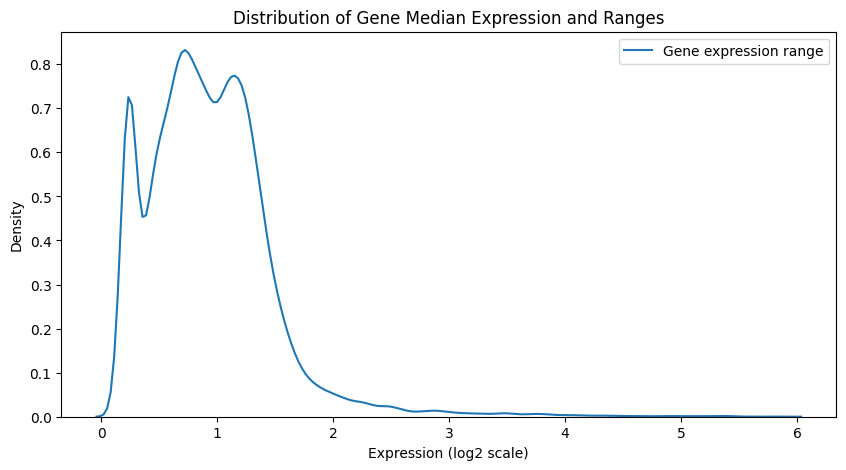
\includegraphics[scale=0.5]{figure_1.png}
\caption{Distribution of gene median expression and ranges}
\label{fig:gene median expression}
\end{figure}
\pagebreak

\item [2.] Now we generate a PCA plot, a T-SNE plot, and a UMAP plot of our data.
	\begin{figure}[h]
\centering
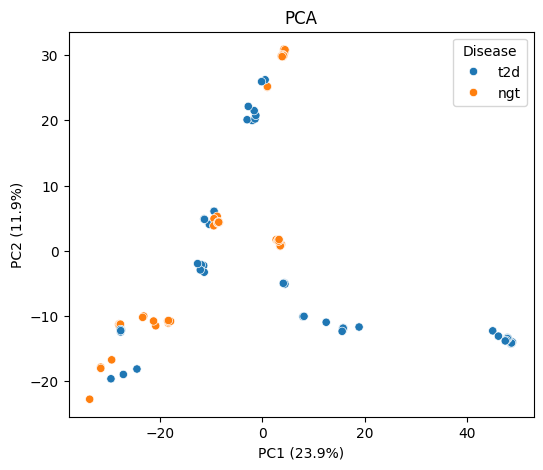
\includegraphics[scale=0.65]{figure_2_pca.png}
\caption{PCA}
\label{fig:pca plot}
\end{figure}
	\begin{figure}[h]
\centering
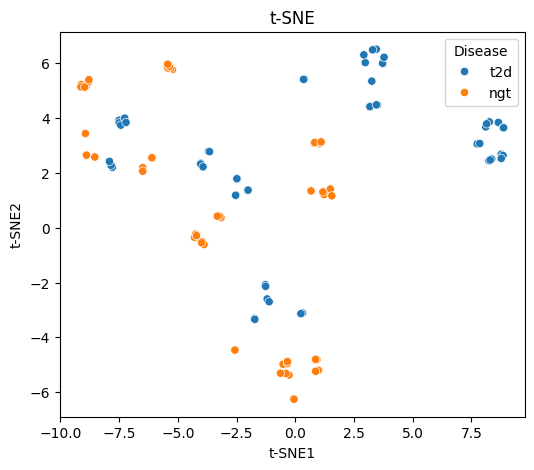
\includegraphics[scale=0.65]{figure_3_tsne.png}
\caption{PCA}
\label{fig:tsne plot}
\end{figure}
	\begin{figure}[h]
\centering
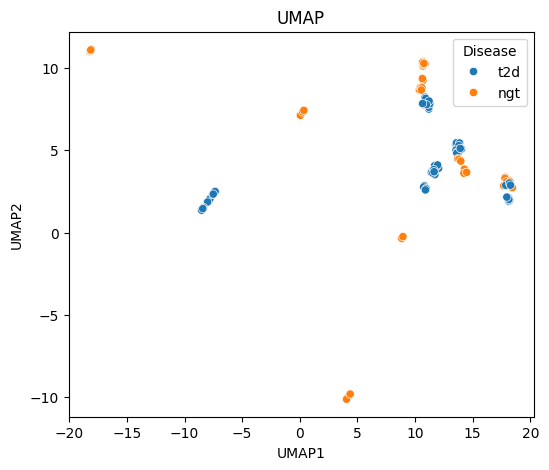
\includegraphics[scale=0.65]{figure_4_umap.png}
\caption{PCA}
\label{fig:umap plot}
\end{figure}

\pagebreak

\item [3.] Volcano plot

	\begin{figure}[h]
\centering
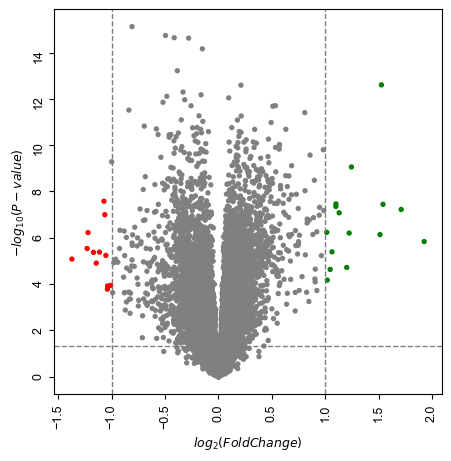
\includegraphics[scale=0.65]{figure_5_volcano_plot.png}
\caption{PCA}
\label{fig:volcano plot}
\end{figure}

\pagebreak

\item [4.] Significant genes

\item [5.] Enrichment analysis



\end{itemize}

\end{document}
